\documentclass{article}

 % Dans le préambule
%\usepackage[style=author]{biblatex} % package de bibliographie, on cite l’auteur
%\addbibresource{Bib2Validation.bib} % notre fichier bib exporté

%%%%% Tous les packages
\usepackage[left=2cm,right=2cm,top=2cm,bottom=2cm]{geometry}
\usepackage[utf8]{inputenc}% accents in
\usepackage[english]{babel}% typo française
\usepackage[T1]{fontenc}% accents out
\usepackage{lmodern}
\usepackage{titlepic}
\usepackage[noae]{Sweave} % "noae" permet à Sweave de reconnaitre les guillemets
\usepackage[%
    all,
    defaultlines=3 % nombre minimum de lignes
]{nowidow} % éviter les lignes orphelines

% package maths
\usepackage{amsmath}
\usepackage{amsfonts}
\usepackage{amssymb}
\usepackage{ dsfont } %proba
\usepackage{ stmaryrd }
% tables et figures
	
\usepackage{subfigure}
\usepackage{lscape}
\usepackage{multirow} % permet de fusionner les colonnes
\usepackage{graphicx} % admet les figures
\usepackage{array} % types particuliers de tableaux
\usepackage{tabularx} % autres tableaux, notamment pour gérer les doubles traits de séparation (voir hhline)
\usepackage{listings} % pas forcément utile ici, mais permet de faire des box avec du code
\usepackage[hang,font = normalsize, labelfont=bf,textfont=bf]{caption} % mise en forme du caption
% hyperlinks
\usepackage{hyperref}
\hypersetup{ %moduler les couleurs des liens
    colorlinks=true,
    linkcolor=black,
    % filecolor=magenta,      
    urlcolor= blue,
}
\usepackage{indentfirst} % Pour indenter les premiers paragraphes de section
%kableExtra
\usepackage{booktabs}
\usepackage{longtable}
\usepackage{array}
\usepackage{multirow}
\usepackage{wrapfig}
\usepackage{float}
\usepackage{colortbl}
\usepackage{pdflscape}
\usepackage{tabu}
\usepackage{threeparttable}
\usepackage{threeparttablex}
\usepackage[normalem]{ulem}
\usepackage{makecell}
\usepackage{xcolor}
%\usepackage[absolute,overlay]{textpos}

% Pour ne pas que la mention "Chapter" apparaisse à chaque chapitre mais juste le titre du chapitre
\usepackage{titlesec}
\titleformat{\chapter}{\normalfont\LARGE}{\thechapter.}{30pt}{\LARGE\bf}
\titleformat{\section}
  {\normalfont\fontsize{15}{15}\bfseries}{\thesection}{1em}{}
\titlespacing*{\chapter}{0pt}{1.1\baselineskip}{\baselineskip}



% Ne pas sauter de page entre deux chapitres





% titres
\title{\centering 

\vspace{1 cm}

{\begin{minipage}\linewidth
        \centering
     \textbf{ Un effet inattendu du confinement : une chute de la surmortalité violente chez les jeunes ?} \\[1 cm] 
        \vspace{0.5cm}
        \large Abel Aussant, Eliot Forcadell et Ariane Sessego\\
         M2 Quantifier en Sciences Sociales\\
        \vspace{0.5cm}
         \textit{Identification causale} Cours d'Olivier Godechot \\
         Année académique 2021-2022\\
    \end{minipage}}
  }
\date{}
%box

\begin{document}
\Sconcordance{concordance:Aussant_Forcadell_Sessego.tex:Aussant_Forcadell_Sessego.Rnw:%
1 116 1 1 19 31 1 1 16 3 1 1 10 1 7 55 1}

\maketitle

\cleardoublepage%

En 2020, les épisodes de confinements ont bouleversé la vie des Français. Ces restrictions de sortie en dehors du domicile avaient pour but de protéger les plus vulnérables du virus de la Covid-19, particulièrement les personnes âgées. Mais on peut se demander s'ils n'ont pas aussi eu des effets inattendus : le confinement a-t-il entrainé une diminution de la mortalité chez les jeunes ? \\

En effet, le risque de décès entre 15 et 30 ans est souvent plus élevé que l'on ne pourrait s'y attendre face à l'augmentation exponentielle de la mortalité habituellement constatée entre 10 et 60 ans (Remund, Camarada, 2021). On désigne donc comme "surmortalité" cet excès par rapport au risque de décès attendu, qui a longtemps été considéré comme uniquement masculin, lié aux turbulences hormonales et de développement biologiques des jeunes hommes\footnote{Heligman L., Pollard J.H., The age pattern of mortality, Journal of the Institute of Actuaries, 1980, 107(1), p. 49-80 et  Goldstein J. A., Secular trend toward earlier male sexual maturity: Evidence from shifting ages of male young adult mortality, PLoS ONE, 2011, 6(8), e14826.}, et liée à des causes violentes de décès (accidents, homicides...). Ces théories développementalistes ont été largement remises en question, du fait des variations de cette tendance dans le temps et l'espace ; cette surmortalité semble avant tout liée à des contexte socio-historiques particulier (Remund, Camarada, 2021). En France aujourd'hui, bien qu'elle touche aussi les jeunes femmes, cette surmortalité est bien plus importante parmi les hommes, avec en moyenne trois fois plus de décès masculins que féminin à ces âges (Breton, Barbieri, 2018). Elle est avant tout caractérisée par une part importante d'accidents de la circulation et de morts violentes (autres types d'accidents, homicides ou suicides) qui sont l'origine de 80\% des décès à ces âges (Remund, Camarada, 2021, trouver une ref plus récente parce parle des années 1960). \\

Le confinement a théoriquement réduit l'exposition à ces risques, à l'exception du suicide. A-t-il entraîné une diminution de la mortalité au sein de cette population ? Le deuxième confinement, moins restrictif que le premier, a-t-il eu un impact plus faible sur cette mortalité ? \\

Pour répondre à ces questions nous utilisons ici une méthode de différence de différence (\textit{diff-in-diff}) pour comparer la mortalité parmi les jeunes adultes en 2020 pendant les périodes de confinement avec celle de 2018 et 2019. En effet, \textit{Présentation succinte de la méthode de diff-in-diff} %Consistant à comparerpour comparer la mortalité parmi les jeunes adultes en 2020, par rapport à celle de 2018 et 2019, pendant les périodes de confinement, nous cherc



\section{Données}

\subsection{Présentation des données INSEE, décès par jour de décès, age et sexe, 2018 à 2020}




\subsection{Quelques statistiques descriptives}





Nombre de décès moyen par jour 2018-2019-2020 (environ 10,4 décès par jour), déviation standard (environ 3,5)
Il faut juste que je mette en forme les données


\begin{center}
\begin{figure}[h!]
\caption{\label{Graph_descr}Tendances mortalité par jour (gaussian smoothing)}
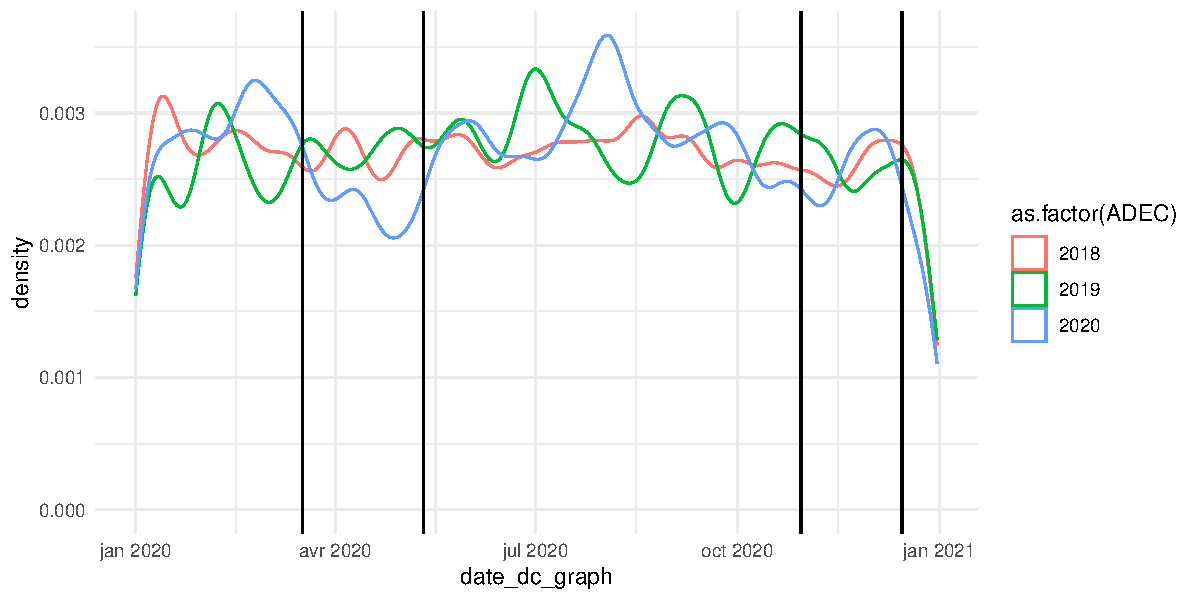
\includegraphics{Aussant_Forcadell_Sessego-003}
\end{figure}
\end{center}








\section{Méthode}

\subsection{La méthode de différence de différence}


\subsection{Les modèles de régressions choisis}

Comparer les périodes de confinements aux tendances de début d'années (on suppose que les jeunes sont peu touchés par le Covid, et que les trends du milieu d'année sont touchées par un effet Covid)\\

- Ajouter un effet année \\

- Ajouter un effet weekend \\

- Se demander si la diminution de la mortalité pendant le confinement n'est pas contrebalancée par une augmentation de la mortalité post-confinement ? (il semblerait que pas totalement)\\





\section{Résultats et Discussion}

Régressions \\


Limites : \\

- Les faibles effectifs font que les tendances sont assez chaotiques, il faudrait comparer sur plus longtemps. \\

- Trop peu d'effectifs pour comparer homme/femme. \\











\end{document}
